\section{Équation de rendu}

L'équation de rendu représente l'impact de la radiance de la lumière sur une surface. En effet, elle va nous permettre de déterminer la manière dont la lumière se reflète sur un objet.

\begin{figure}[H]
	\bounce
	\centering 
	\captionof{figure}{Schéma de la réflection total des rayons de directions $\omega_i$ résultant en un rayon de direction $\omega_o$ sur le point $x$ d'une surface.}
\end{figure}

L'équation de rendu se définie comme suit (cf démonstration en Annexe 1):

$$\boxed{L_{o}(x, \omega_o) = L_{e}(x, \omega_o) + \int_{\Omega}f(x, \omega_o, \omega_i) \, L_{i}(x, \omega_i) \, \cos\left(\theta_i\right) \, d_{\omega_i}}$$

avec: 
\begin{itemize}
\item[$\_$] $\overrightarrow{n}$ : La normale de la surface au point $x$.
\item[$\_$] $\Omega$ : L'hémisphère centré autour de la normale $\textbf{n}$.
\item[$\_$] $x$ : Le point de $\mathbb{R}^3$ d'intersection entre les rayons incidents et la surface de l'objet considéré.
\item[$\_$] $\overrightarrow{\omega_o}$ : Direction du rayon réfléchis dans $\Omega$ sur la surface au point $x$.
\item[$\_$] $\overrightarrow{\omega_i}$ : Directions des rayons incidents dans $\Omega$ sur la surface au point $x$.
\item[$\_$] $L_o$ : La radiance réfléchis sur la surface au point $x$ de direction $\overrightarrow{\omega_o}$.
\item[$\_$] $L_e$ : La radiance émise par la surface au point $x$ de direction $\overrightarrow{\omega_o}$.
\item[$\_$] $L_i$ : Les radiances des rayons incidents sur la surface au point $x$ de direction $\overrightarrow{\omega_i}$.
\item[$\_$] $f$ : Le BRDF qui représente la manière dont le matériaux reflète la lumière.
\end{itemize}

\subsection{Les matériaux Lambertiens}

Cette équation n'est pas résoluble analytiquement. Pour faciliter les calculs et l'implémentation de notre path tracing, nous allons nous prendre le cas des matériaux dit "Lambertiens".\\

Ce type de matériaux inclus tous les matériaux de surface rugueuse qui n'émettent pas dans la lumière visible. Nous pouvons donc simplifier l'équation de rendu avec (cf démonstration Annexe 1):


$$ 
\boxed{L_o(x, \omega) = \frac\rho\pi \int_\Omega L_i(x, \omega_i) \, \cos\left(\theta_i\right) \, d_{\omega_i}}
$$

\subsection{Approximation avec la méthode Monte-Carlo}

La méthode de Monte-Carlo est une méthode itérative permettant de passer d'une intégrale à une somme d'échantillons aléatoires pondérée par une loi de probabilité notée $pdf$ (Probability Density Function). Cette somme converge vers la solution vraie en fonction du nombre d'échantillons.

Ainsi, nous avons l'approximation suivante:

Soit g, une fonction telle que: $g:\ \left\{
\begin{array}{l}
\mathbb{R} \longmapsto \mathbb{R}\\
x\longrightarrow g(x)
\end{array}
\right.$:
$$
I = \int_\Omega g(x) \, d_x \approx \frac{1}{N} \sum_k^N \frac{g(x_k)}{pdf(x_k)}
$$
\subsubsection{Méthode d'échantillonnage Cosine-Weighted} 

Pour des matériaux lambertiens, nous choisissons un échantillonnage dit "Cosine-weighted". Il consiste à se placer dans le repère local $(tangente, bitangente, normal)$ au point d'intersection (cf. \textit{Figure 9}), pour ensuite construire le rayon aléatoire.\\

\begin{figure}[H]
	\centering
\begin{minipage}{.4\textwidth}
	
	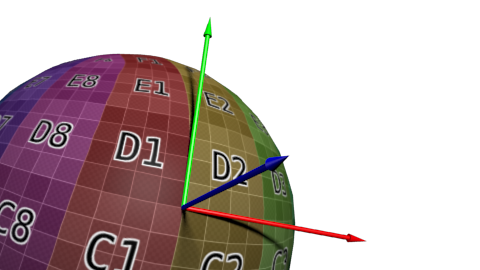
\includegraphics[scale=0.5]{include/NTBFromUVs.png}
\end{minipage}
\captionof{figure}{Représentation de la base locale au point d'intersection du rayon sur la sphère
avec la normale (en bleu), la bitangente (en vert) et la tangente (en rouge).}
\small{Source: https://www.opengl-tutorial.org/fr/intermediate-tutorials/tutorial-13-normal-mapping/}
\end{figure}

 Ce mode d'échantillonnage se fait de la manière suivante:
\begin{itemize}
\item[$\_$] Génération de 2 nombres aléatoires $\xi_1\in\mathbb{N}$ et $\xi_2\in\mathbb{N}$\\
\item[$\_$] On les passe en coordonnées polaires: $\left\{
\begin{array}{l}
r = \sqrt{\xi_1}\\
\theta = 2\pi\xi_2
\end{array}
\right.$
\item[$\_$] On passe les coordonnées polaires dans la base locale:$\left\{
\begin{array}{l}
x = r\cos\theta\\
y = r\sin\theta\\
z = \sqrt{1-r^2}
\end{array}
\right.$\\

\end{itemize} 
Ainsi, on construit la direction du rayon incident $\omega_i$ de la manière suivante dans la base $\left( right, up, forward\right)$: $\omega_i = x\cdot tangente + y\cdot bitangente+ z\cdot normal $.\\

L'avantage de cette méthode d'échantillonnage est que la $pdf$ sera: $pdf = \frac{\cos\theta_i}{\pi}$.

\subsubsection{Application de la Méthode de Monte-Carlo pour l'équation de rendu}

L'équation de rendu avec la méthode de Monte-Carlo s'écrit de la façon suivante:
\\
$$ 
L_o(x, \omega_o) = \frac\rho\pi \sum_{i=1}^N \frac{L_i(x, \omega_i) \, \cos\left(\theta_i\right)}{pdf(\omega_i)}
$$

$$ 
L_o(x, \omega_o) = \rho\sum_{i=1}^N {L_i(x, \omega_i)}
$$
\\

Ainsi, nous avons pu bien simplifier l'équation de rendu en choisissant le bon échantillonnage et en travaillant sur les bons matériaux.

\subsection{Implémentation}
Le choix que nous avons fait pour notre première version naïve est la suivante: la somme $\rho\sum_{i=1}^N {L_i(x, \omega_i)}$ est représentée dans notre code comme étant une fonction récursive. En effet, pour chaque rebond, nous allons sommer $\rho\ L_i(x, \omega_i)$ et retourner le résultat pour chaque échantillon de pixel. La fonction sera de la manière suivante:

\begin{algorithm}[H]
\caption{Échantillonnage récursif d’un rayon (RaySampling)}
\begin{algorithmic}[1]
\Require Rayon $r$, scène $S$, caméra $cam$, profondeur $d$, profondeur max $d_{\max}$
\Ensure Couleur incidente $L$
\State Initialiser $L \gets (0,0,0)$
\State $black \gets (0,0,0)$
\If{$d = d_{\max}$}
    \State \Return $black$
\EndIf
\If{pas d’intersection de $r$ avec la scène}
  \State \Return couleur de fond de la scène
\EndIf
\If{l’objet est émissif}
    \State $L \gets intensite \cdot couleur\_objet$
    \State \Return $L$
\EndIf
\State Générer un rayon réfléchi $r_{new}$ dans l’hémisphère selon une loi Cosine-Weighted

\State $L_{ref} \gets$ \Call{RaySampling}{$r_{new}, S, cam, d+1, d_{\max}$}
\State$L \gets L+albedo \cdot L_{ref}$
\State \Return $L$

\end{algorithmic}
\end{algorithm}



\pagebreak
